\let\negmedspace\undefinedx
\let\negthickspace\undefined
\documentclass[journal]{IEEEtran}
\usepackage[a5paper, margin=10mm, onecolumn]{geometry}
%\usepackage{lmodern} % Ensure lmodern is loaded for pdflatex
\usepackage{tfrupee} % Include tfrupee package

\setlength{\headheight}{1cm} % Set the height of the header box
\setlength{\headsep}{0mm}     % Set the distance between the header box and the top of the text

\usepackage{gvv-book}
\usepackage{gvv}
\usepackage{cite}
\usepackage{amsmath,amssymb,amsfonts,amsthm}
\usepackage{algorithmic}
\usepackage{graphicx}
\usepackage{textcomp}
\usepackage{xcolor}
\usepackage{txfonts}
\usepackage{listings}
\usepackage{enumitem}
\usepackage{mathtools}
\usepackage{gensymb}
\usepackage{comment}
\usepackage[breaklinks=true]{hyperref}
\usepackage{tkz-euclide} 
\usepackage{listings}
% \usepackage{gvv}                                        
\def\inputGnumericTable{}                                 
\usepackage[latin1]{inputenc}                                
\usepackage{color}                                            
\usepackage{array}                                            
\usepackage{longtable}                                       
\usepackage{calc}                                             
\usepackage{multirow}                                         
\usepackage{hhline}                                           
\usepackage{ifthen}                                           
\usepackage{lscape}


\renewcommand{\thefigure}{\theenumi}
\renewcommand{\thetable}{\theenumi}
\setlength{\intextsep}{10pt} % Space between text and floats


\numberwithin{equation}{enumi}
\numberwithin{figure}{enumi}
\renewcommand{\thetable}{\theenumi}

% Marks the beginning of the document
\begin{document}
\bibliographystyle{IEEEtran}

\title{Assignment 5}
\author{EE24BTECH11049 \\ Patnam Shariq Faraz Muhammed}

% \maketitle
% \newpage
% \bigskip
{\let\newpage\relax\maketitle}
\section{Carry TWO marks Each}
\begin{enumerate}
		%1st Question 
	\item A student performed X-rays diffraction experiment on a FCC polycrystalline pure metal. The following $\sin^{2}{\theta}$ values were calculated from the diffraction peaks. 
		\begin{align*}
			\sin^{2}{\theta} = 0.136, 0.185, 0.504, 0.544
		\end{align*}
	However, the student was negligent and missed noting one of the peaks. Which one of the following Miller indices corresponds to the missing peak? 
		
		\hfill{\brak{\text{XE 2023}}}

		\begin{multicols}{4}
			\begin{enumerate}
				\item $\brak{200}$
				\item $\brak{220}$
				\item $\brak{311}$
				\item $\brak{222}$
			\end{enumerate}
		\end{multicols}

		%2nd Question 
	\item Match the lattice planes and directions \brak{\text{in Column }\mathrm{I}} with the corresponding Miller indices \brak{\text{in Column }\mathrm{I}}
		\begin{multicols}{2}
			\textbf{Column} $\mathrm{I}$ 
			\begin{enumerate}
				\item[(P)] 
					\centering
					\resizebox{0.35\columnwidth}{!}{\begin{tikzpicture}
    % Define points for the cube
    \coordinate (A) at (0,0);
    \coordinate (B) at (2,0);
    \coordinate (C) at (2,2);
    \coordinate (D) at (0,2);
    \coordinate (E) at (1,1);
    \coordinate (F) at (3,1);
    \coordinate (G) at (3,3);
    \coordinate (H) at (1,3);

    % Draw edges of the cube
    \draw[thick] (A) -- (B) -- (C) -- (D) -- (A); % Bottom square
    \draw[thick] (E) -- (F) -- (G) -- (H) -- (E); % Top square
    \draw[thick] (A) -- (E); % Left edge
    \draw[thick] (B) -- (F); % Right edge
    \draw[thick] (C) -- (G); % Top right edge
    \draw[thick] (D) -- (H); % Top left edge
    \draw[->,thick](A) -- (1.5,2.5);
    % Labels
    \node[below left, scale=2] at (A) {$a$};
    \node[below right, scale=2] at (B) {$b$};
    \node[above, scale=2] at (G) {$c$};
\end{tikzpicture}
}
				\item[(Q)]
                                        \centering
                                        \resizebox{0.35\columnwidth}{!}{\begin{tikzpicture}
    % Define points for the cube
    \coordinate (A) at (0,0);
    \coordinate (B) at (2,0);
    \coordinate (C) at (2,2);
    \coordinate (D) at (0,2);
    \coordinate (E) at (1,1);
    \coordinate (F) at (3,1);
    \coordinate (G) at (3,3);
    \coordinate (H) at (1,3);

    % Draw edges of the cube
    \draw[thick] (A) -- (B) -- (C) -- (D) -- (A); % Bottom square
    \draw[thick] (E) -- (F) -- (G) -- (H) -- (E); % Top square
    \draw[thick] (A) -- (E); % Left edge
    \draw[thick] (B) -- (F); % Right edge
    \draw[thick] (C) -- (G); % Top right edge
    \draw[thick] (D) -- (H); % Top left edge
    \draw[thick] (B) -- (E) -- (H) -- (C) -- (B);

    % Labels
    \node[below left, scale=2] at (A) {$a$};
    \node[below right, scale=2] at (B) {$b$};
    \node[above, scale=2] at (G) {$c$};
\end{tikzpicture}
}
				\item[(R)]
                                        \centering
                                	\resizebox{0.35\columnwidth}{!}{\begin{tikzpicture}
    % Define points for the cube
    \coordinate (A) at (0,0);
    \coordinate (B) at (2,0);
    \coordinate (C) at (2,2);
    \coordinate (D) at (0,2);
    \coordinate (E) at (0.8,0.8);
    \coordinate (F) at (3,0.8);
    \coordinate (G) at (3,3);
    \coordinate (H) at (0.8,3);

    % Draw edges of the cube
    \draw[thick] (A) -- (B) -- (C) -- (D) -- (A); % Bottom square
    \draw[thick] (E) -- (F) -- (G) -- (H) -- (E); % Top square
    \draw[thick] (A) -- (E); % Left edge
    \draw[thick] (B) -- (F); % Right edge
    \draw[thick] (C) -- (G); % Top right edge
    \draw[thick] (D) -- (H); % Top left edge
    \draw[thick] (D) -- (E) -- (B) -- (D);

    % Labels
    \node[below left, scale=2] at (A) {$a$};
    \node[below right, scale=2] at (B) {$b$};
    \node[above, scale=2] at (G) {$c$};
\end{tikzpicture}
}
				\item[(S)]
                                        \centering
                                        \resizebox{0.35\columnwidth}{!}{\begin{tikzpicture}
    % Define points for the cube
    \coordinate (A) at (0,0);
    \coordinate (B) at (2,0);
    \coordinate (C) at (2,2);
    \coordinate (D) at (0,2);
    \coordinate (E) at (1,1);
    \coordinate (F) at (3,1);
    \coordinate (G) at (3,3);
    \coordinate (H) at (1,3);

    % Draw edges of the cube
    \draw[thick] (A) -- (B) -- (C) -- (D) -- (A); % Bottom square
    \draw[thick] (E) -- (F) -- (G) -- (H) -- (E); % Top square
    \draw[thick] (A) -- (E); % Left edge
    \draw[thick] (B) -- (F); % Right edge
    \draw[thick] (C) -- (G); % Top right edge
    \draw[thick] (D) -- (H); % Top left edge
    \draw[->,thick](A) -- (3,2);
    % Labels
    \node[below left, scale=2] at (A) {$a$};
    \node[below right, scale=2] at (B) {$b$};
    \node[above, scale=2] at (G) {$c$};
\end{tikzpicture}
}
			\end{enumerate}
			\columnbreak
			\textbf{Column} $\mathrm{II}$
			\begin{enumerate}
				\item[1] $\brak{\overline{1}11}$
				\item[2] $\brak{\overline{1}12}$
				\item[3] $\brak{\overline{2}21}$
				\item[4] $\brak{\overline{1}10}$
			\end{enumerate}
		\end{multicols}

		\hfill{\brak{\text{XE 2023}}}

		\begin{enumerate}
			\item P-2, Q-4, R-1, S-3 
			\item P-3, Q-1, R-4, S-2
			\item P-2, Q-4, R-3, S-1
			\item P-3, Q-4, R-2, S-1
		\end{enumerate}

		%3rd Question 
	\item Match the hardness test \brak{\text{in Column }\mathrm{I}} with its indenter type \brak{\text{in Column }\mathrm{II}}
		\begin{multicols}{2}
			\textbf{Column} $\mathrm{I}$
			\begin{enumerate}
				\item [P] Brinell
				\item [Q] Rockwell
				\item [R] Vickers
			\end{enumerate}
			\columnbreak
			\textbf{Column} $\mathrm{II}$
			\begin{enumerate}
				\item[1] Diamond pyramidal
				\item[2] Diamond cone
				\item[3] Tungsten carbide sphere
				\item[4] Steel sphere
			\end{enumerate}
		\end{multicols}

		\hfill{\brak{\text{XE 2023}}}

		\begin{enumerate}
			\item P-2, Q-4, R-1
			\item P-4, Q-2, R-3
			\item P-3, Q-4, R-2
			\item P-4, Q-2, R-1
		\end{enumerate}

		%4th Question 
	\item TTT diagram of a eutectoid steel is shown below. Match the heat treatment cycle \brak{\text{in Column }\mathrm{I}} with its microstructure \brak{\text{in Column }\mathrm{II}}
		
		\begin{figure}[H]
			\centering 
			\resizebox{0.5\textwidth}{!}{\begin{circuitikz}
\tikzstyle{every node}=[font=\large]
\draw  (1.75,11) rectangle (9,4.25);
\draw [dashed] (1.75,10.5) -- (9,10.5);
\draw [dashed] (1.75,5) -- (9,5);
\draw [dashed] (1.75,5.75) -- (9,5.75);
\draw [->, >=Stealth, dashed] (3.5,6) -- (7.75,6);
\draw [->, >=Stealth, dashed] (4.5,8.5) -- (5.5,4.5);
\draw [->, >=Stealth, dashed] (3.25,9.25) -- (7.5,9.25);
\draw [dashed] (4.5,8.5) -- (2.75,8.5);
\draw [dashed] (2.75,8.5) -- (2.25,10.75);
\draw [dashed] (3.25,9.25) -- (3,10.75);
\draw [dashed] (2.5,10.75) -- (3.5,6);
\node [font=\large] at (5,4) {$Time(s)$};
\node [font=\large, rotate around={90:(0,0)}] at (1.5,8) {$Temperature\brak{^{\degree}C}$};
\node [font=\large] at (8,6) {R};
\node [font=\large] at (7.75,9.25) {P};
\node [font=\large] at (5.75,4.5) {Q};
\node [font=\large] at (1.25,10.5) {727};
\node [font=\large] at (1.5,5) {$M_f$};
\node [font=\large] at (1.5,5.75) {$M_s$};
\node [font=\large] at (4.5,10.75) {Austenite};
\end{circuitikz}
}
		\end{figure}

		\begin{multicols}{2}
			\textbf{Column} $\mathrm{I}$
			\begin{enumerate}
				\item P
				\item Q
				\item R
			\end{enumerate}
			\columnbreak
                        \textbf{Column} $\mathrm{II}$
			\begin{enumerate}
				\item[1] Bainite only
				\item[2] Pearlite only
				\item[3] Pearlite + Bainite + Martensite
				\item[4] Pearlite + Martensite
			\end{enumerate}
		\end{multicols}

		\hfill{\brak{\text{XE 2023}}}

		\begin{enumerate}
			\item P-1, Q-2, R-4
			\item P-2, Q-3, R-2
			\item P-2, Q-4, R-1
			\item P-2, Q-3, R-1
		\end{enumerate}

		%5th Question
	\item Which of the following statement\brak{\text{s}} is/are true for an optical microscope?
		
		\hfill{\brak{\text{XE 2023}}}

		\begin{enumerate}
			\item Increasing the aperture of the objective lens deteriorates the resolution
			\item Reducing the wavelength of illuminating light improves the resolution
			\item Increasing the refractive index of the medium in between the sample and the objective lens improves the resolution
			\item Reducing the wavelength of illuminating light decreases the depth of field
		\end{enumerate}

		%6th Question 
	\item Among the 14 Bravais lattices, there is no base centred cubic unit cell. Which of the following statement\brak{\text{s}} is/are true?
		
		\hfill{\brak{\text{XE 2023}}}

		\begin{enumerate}
			\item The base-centred cubic unit cell is same as the simple tetragonal unit cell
			\item The base-centred cubic unit cell is same as the body centred tetragonal unit cell
			\item The base-centred cubic unit cell is same as the simple orthorhombic unit cell
			\item The base-centred cubic unit cell does not have any 3-fold rotation axis
		\end{enumerate}

		%7th Question 
	\item Specific heat $\brak{C_v}$ of a material was found to depend on temperature as shown below. Which of the following statement\brak{\text{s}} is/are true 

		\begin{figure}[H]
			\centering
			\resizebox{0.6\textwidth}{!}{\begin{circuitikz}
\tikzstyle{every node}=[font=\large]
\draw [line width=0.9pt, ->, >=Stealth] (2.25,6) -- (2.25,10);
\draw [line width=0.9pt, ->, >=Stealth] (2.25,6) -- (7,6);
\draw [line width=0.9pt, short] (2.25,8.25) -- (6,9.75);
\node [font=\large] at (1.5,9) {$\frac{C_v}{T}$};
\node [font=\normalsize, rotate around={90:(0,0)}] at (1.75,7.25) {$\brak{J-kg^{-1}-K^{-2}}$};
\node [font=\large] at (4.5,5.5) {$T^2 \brak{K^2}$};
\end{circuitikz}
}
		\end{figure}

		\hfill{\brak{\text{XE 2023}}}

		\begin{enumerate}
			\item The material is metallic
			\item The material is insulating
			\item The material is three dimensional
			\item The material is one dimensional
		\end{enumerate}

		%8th Question 
	\item A pure Silicon wafer is doped with Boron by exposing it to $B_2O_3$ vapour at an elevated temperature. It takes 1000 seconds to reach a Boron concentration of $10^{20} atoms-m^{-3}$ at a depth of $1\mu m$ is \brak{\text{in seconds}}:\rule{1cm}{0.1pt} \brak{\text{rounded off to nearest integer}}

		Given: Boron concentration on the wafer surface remains constant.

		\hfill{\brak{\text{XE 2023}}}

		%9th Question
	\item The Young's modulus of a quartz piezoelectric crystal is $100GPa$. The uniaxial stress required to change its polarization by $\%$ is \brak{\text{give absolute value in }GPa}\rule{1cm}{0.1pt} \brak{\text{rounded off to nearest integer}} 

		\hfill{\brak{\text{XE 2023}}}

		%10th Question 
	\item A one-dimensional nanowire has a linear electron density of $10^8 electrons-cm^{-1}$. The Fermi energy of the system is \brak{\text{in } eV}\rule{1cm}{0.1pt} \brak{\text{rounded off to two decimal places}}

		Given: $\frac{\hbar^2}{2m} = 0.24\brak{eV}^2-s^2-kg^{-1}$ where $'m'$ is the mass of an electron

		\hfill{\brak{\text{XE 2023}}}

		%11th Question 
	\item Two moles of a monoatomic ideal gas at $10 atm$ and $300 K$ is expanded isothermally and reversibly to a pressure of $2 atm$. The absolute value of work done by the system is \brak{\text{in kJ}} \rule{1cm}{0.1pt} \brak{\text{rounded off to two decimal places}}

		Given: R = $8.31J-mol^{-1}K^{-1}$, $1 atm = 101 kPa$

		\hfill{\brak{\text{XE 2023}}}

		%12th Question 
	\item An electrochemical cell consists of pure $Zn$ electrode \brak{\text{anode}} and a hydrogen electrode \brak{\text{cathode}} in dilute $Zn^{+2}$ solution. The overall reaction: 
		\begin{align*}
			Zn\brak{s} + 2H^{+} \rightleftharpoons H_2 + Zn^{+2}
		\end{align*}
		If the overall cell potential is $+0.690 V$, then the value of $\ln{\frac{\brak{\sbrak{Zn^{+2}}}}{\sbrak{H^{+}}^2}}$ is \rule{1cm}{0.1pt} \brak{\text{rounded off to two decimal places}}
		Given: Pressure of hydrogen gas $= 1 atm$; Temperature $= 298K$;
		$\frac{RT}{F} = 0.0256 V$, where $R$ is gas constant and $F$ is Faraday constant
		The standard reduction potential of: 
		\begin{align*}
			Zn^{+2} + 2e \rightarrow Zn \brak{E^{\degree} = -0762 V} \text{ versus Standard Hydrogen Electrode } \\
			2H^{+} + 2e \rightarrow H_2 \brak{E^{\degree} = 0 V}
		\end{align*}

		\hfill{\brak{\text{XE 2023}}}

		%13th Question 
	\item In a Raman spectroscopy experiment done at $300K$, a Raman line is observed at $200cm^{-1}$\brak{25 meV}. The ratio of the intensity of the Stokes line to that of the Anti-Stokes line is \rule{1cm}{0.1pt} \brak{\text{rounded off to two decimal places}}

		Given: Boltzmann constant, $k = 8.62 \times 10^{-5} eV-K^{-1}$
		\hfill{\brak{\text{XE 2023}}}
\end{enumerate}
\end{document}
